\documentclass{beamer}
\usetheme{CMU}

\usepackage{slpython}
\usepackage{underscore}

\usepackage{pgf,pgfarrows,pgfnodes,pgfautomata,pgfheaps,pgfshade}
\usepackage{amsmath,amssymb}
\usepackage[utf8]{inputenc}
\usepackage{colortbl}
\usepackage[english]{babel}
\usepackage{booktabs}

\newcommand*{\True}{\mbox{True}}
\newcommand*{\False}{\mbox{False}}
\newcommand*{\Expected}{\ensuremath{\mathbb{E}}}
\newcommand{\pd}[2]{\frac{\partial#1}{\partial#2}}
\newcommand{\pdd}[2]{\frac{\partial^2 #1}{\partial #2^2}} 

\newcommand*{\error}[1]{{\color{red}\textbf{#1}}}
\newcommand*{\Assign}{\ensuremath\,:=\,}
\newcommand*{\Dkl}{\ensuremath{D_{\text{\textsc{kl}}}}}
\newcommand*{\vect}[1]{{\vec{#1}}}

\title{Jug: Coarse-Level Parallel Python}
\author{Lu\'\i{}s Pedro Coelho}
\institute{Joint \textsc{cmu}-Pitt PhD.\ in Computational Biology}
%\date{}

\graphicspath{{figures/}{figures/generated/}{../images/}}

\AtBeginSection[] % Do nothing for \subsection*
{
	\begin{frame}<beamer>
		\frametitle{Outline}
		\tableofcontents[currentsection,currentsubsection]
	\end{frame}
}


\begin{document}
\frame{\titlepage}
\begin{frame}[fragile]
\frametitle{Problem}
Cluster a set of images.
\end{frame}

\begin{frame}[fragile]
\frametitle{Simple Solution}

\begin{python}
imgs = glob('*.png')
features = [computefeatures(img,parameter=2)
                for img in imgs]
clusters = []
bics = []
for k in xrange(2,200):
    for seed in xrange(10):
        clusters.append(kmeans(features,k=k,seed=seed))
        bics.append(compute_bic(clusters[-1]))
Nr_clusters = argmin(bics) // 10
\end{python}
\end{frame}

\begin{frame}[fragile]
\frametitle{Use Cluster}

\begin{block}{Individual Scripts}
\begin{enumerate}
\item computefeatures.py IMG PARAMETERS\\
    generates files like \textit{feats_img0_param0_param1.pp}.
\item cluster.py NRCLUSTER SEED\\
    generates files like \textit{clusters_K_seed.pp}
\item pickbestcluster.py
\end{enumerate}
\pause
\begin{enumerate}
\item runcomputefeatures.py
\item runcluster.py
\end{enumerate}
\end{block}

Too fragmented!
\note{too many jobs.

too many intermediate files.
}
\end{frame}

\begin{frame}[fragile]
\frametitle{Use Cluster (II)}
\begin{block}{Coarse Level Scripts}
\begin{enumerate}
\item computefeatures.py IMG0 IMG1 IMG2 IMG3 \dots
\item cluster.py NRCLUSTER0 NRCLUSTER1 NRCLUSTER2 \dots
\item pickcluster.py
\end{enumerate}
\pause
\begin{enumerate}
\item runcomputefeatures.py
\item runclustering.py
\end{enumerate}
\end{block}

\pause
\begin{itemize}
\item \textbf{Pro:} Better use of cluster.
\item \textbf{Cons:} Complex code, very error-prone.
\end{itemize}
\end{frame}

\begin{frame}[fragile]

\begin{columns}[c]
\column{.5\textwidth}
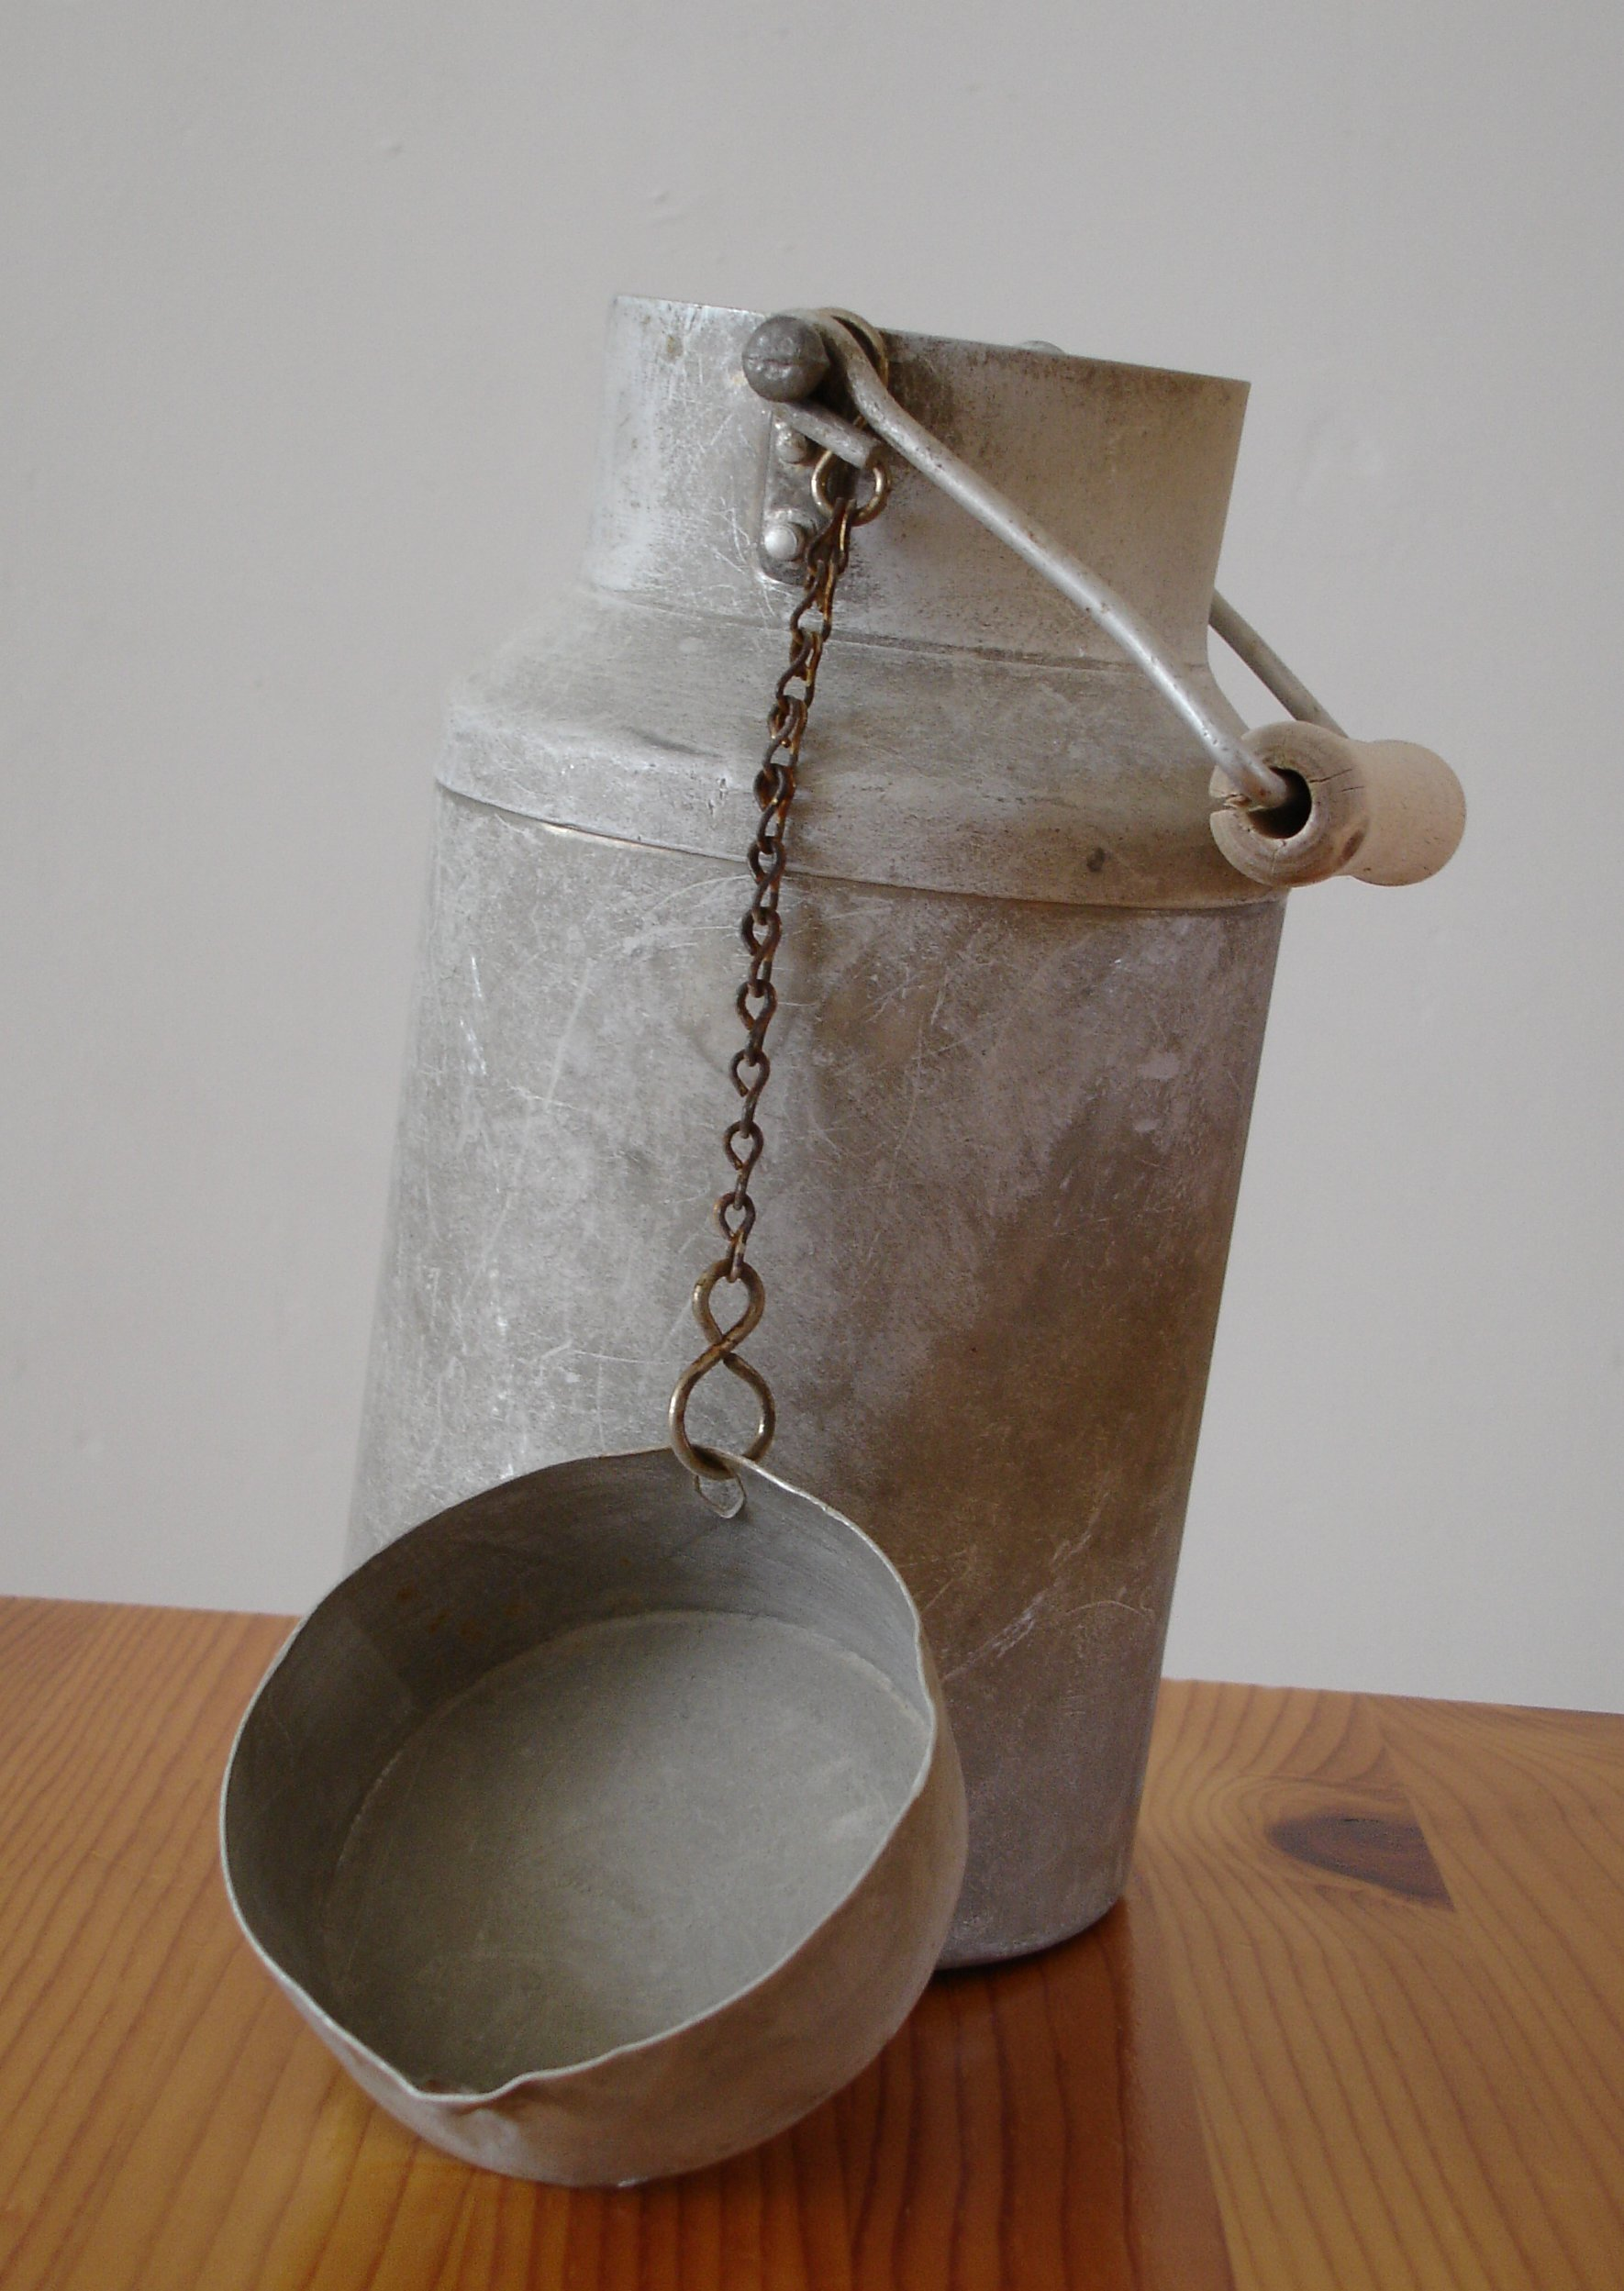
\includegraphics[height=.9\textheight]{brocalait}
% http://commons.wikimedia.org/wiki/File:Broc_%C3%A0_lait.jpg

\column{.5\textwidth}
Jug solves all of these problems!

\end{columns}
\end{frame}

\begin{frame}[fragile]
\frametitle{Tasks}
\begin{python}
imgs = glob('*.png')
feature_tasks = [Task(computefeatures,img,parameter=2)
                    for img in imgs]
cluster_tasks = []
bic_tasks = []
for k in xrange(2,200):
    for seed in xrange(10):
        cluster_tasks.append(
            Task(kmeans,feature_tasks,k=k,seed=seed)
            )
        bic_tasks.append(
            Task(compute_bic,cluster_tasks[-1])
            )
Nr_clusters = Task(argmin,bic_tasks)
\end{python}
\end{frame}

\begin{frame}[fragile]
\frametitle{Python Magic}

\begin{python}
from jug.task import TaskGenerator

computefeatures = TaskGenerator(computefeatures)
kmeans = TaskGenerator(kmeans)
compute_bic = TaskGenerator(compute_bic)

@TaskGenerator
def Nr_Clusters(bics):
    return argmin(bics) // 10

...
\end{python}
\end{frame}

\begin{frame}[fragile]
\frametitle{Python Magic (II)}

\begin{python}
...

imgs = glob('*.png')
features = [computefeatures(img,parameter=2)
            for img in imgs]
clusters = []
bics = []
for k in xrange(2,200):
    for seed in xrange(10):
        clusters.append(kmeans(features,k=k,seed=seed))
        bics.append(compute_bic(clusters[-1]))
Nr_clusters(bics)
\end{python}

\note{Save this as jugfile.py.}
\end{frame}

\begin{frame}[fragile]
\frametitle{Enter Jug}

You give it the Jugfile, it runs the tasks for you!

\end{frame}
\begin{frame}[fragile]
\frametitle{Jug Loop}

\begin{python}
while len(tasks) > 0:
    ready = [t for t in tasks if can_run(t)]
    for t in ready:
        if not is_running(t):
            t.run()
        tasks.remove(t)
\end{python}

We're back where we started!

\end{frame}

\begin{frame}[fragile]
\frametitle{Jug Advantages}
\begin{enumerate}
\item Automatic task-level parallelization with dependency tracking.
\item Remember all intermediate results.
\item Makes writing parallel code look like writing sequential code.
\end{enumerate}
\end{frame}

\begin{frame}[fragile]
\frametitle{Jug Limitations}
\begin{enumerate}
\item This is still \alert{Python}, not a true parallel programming language.
\item It makes it too easy to fill up your hard disk.
\item It is coarse level parallelization.
\end{enumerate}
\end{frame}

\begin{frame}[fragile]
\frametitle{Come Learn Python}

\begin{itemize}
\item \textit{Programming for Scientists}.
\item Course Number: 98-111.
\item Tue \& Thu 6.30--7.20pm SH220.
\end{itemize}
\end{frame}

\end{document}

